\documentclass[border=2pt]{standalone}
\usepackage[T1]{fontenc}
\usepackage{tikz}
\usetikzlibrary{shapes.geometric, arrows.meta, positioning, backgrounds, fit, calc}
\usepackage{amsmath}

\begin{document}
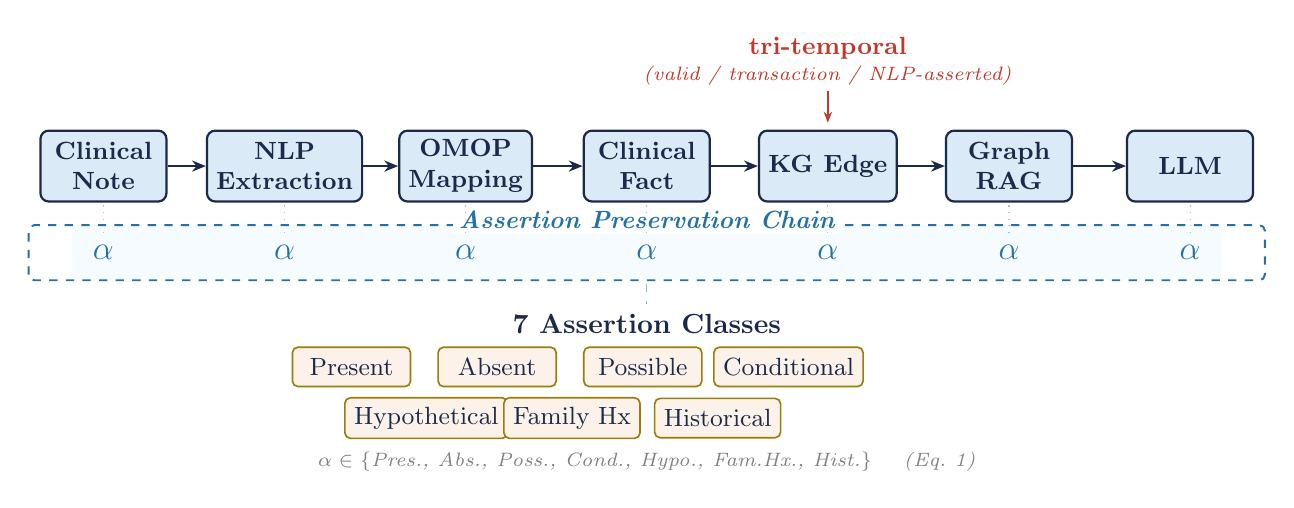
\begin{tikzpicture}[
    % Styles
    pipeline/.style={
        rectangle, rounded corners=3pt,
        draw=darkblue, fill=lightblue,
        line width=0.8pt,
        minimum width=1.6cm, minimum height=0.9cm,
        font=\small\bfseries, text=darkblue,
        align=center
    },
    arrow/.style={
        -{Stealth[length=5pt, width=4pt]},
        line width=0.9pt, color=darkblue
    },
    assertion/.style={
        rectangle, rounded corners=2pt,
        draw=darkgold, fill=warmcream,
        line width=0.6pt,
        minimum width=1.5cm, minimum height=0.5cm,
        font=\small, text=darkblue,
        align=center
    },
]
% Define colors
\definecolor{darkblue}{RGB}{27,42,74}
\definecolor{lightblue}{RGB}{218,234,246}
\definecolor{medblue}{RGB}{36,113,163}
\definecolor{accentred}{RGB}{192,57,43}
\definecolor{darkgold}{RGB}{154,125,10}
\definecolor{warmcream}{RGB}{253,242,233}
\definecolor{chainbg}{RGB}{240,248,255}

% Pipeline boxes
\node[pipeline] (note) at (0,0) {Clinical\\Note};
\node[pipeline] (nlp) at (2.3,0) {NLP\\Extraction};
\node[pipeline] (omop) at (4.6,0) {OMOP\\Mapping};
\node[pipeline] (fact) at (6.9,0) {Clinical\\Fact};
\node[pipeline] (edge) at (9.2,0) {KG Edge};
\node[pipeline] (rag) at (11.5,0) {Graph\\RAG};
\node[pipeline] (llm) at (13.8,0) {LLM};

% Arrows
\draw[arrow] (note) -- (nlp);
\draw[arrow] (nlp) -- (omop);
\draw[arrow] (omop) -- (fact);
\draw[arrow] (fact) -- (edge);
\draw[arrow] (edge) -- (rag);
\draw[arrow] (rag) -- (llm);

% Tri-temporal annotation
\node[font=\small\bfseries, text=accentred, align=center] (tritmp) at (9.2, 1.5) {tri-temporal};
\node[font=\scriptsize, text=accentred, align=center] at (9.2, 1.15) {\textit{(valid / transaction / NLP-asserted)}};
\draw[-{Stealth[length=4pt, width=3pt]}, line width=0.8pt, color=accentred] (9.2, 0.95) -- (9.2, 0.55);

% Assertion Preservation Chain
\begin{scope}[on background layer]
    \node[rectangle, rounded corners=2pt, fill=chainbg, fill opacity=0.6,
          minimum width=14.6cm, minimum height=0.7cm] at (6.9, -1.1) {};
\end{scope}
\draw[dashed, color=medblue, line width=0.7pt, rounded corners=2pt]
    (-0.95, -1.45) rectangle (14.75, -0.75);

% Chain label
\node[font=\small\bfseries\itshape, text=medblue, fill=white, inner sep=2pt]
    at (6.9, -0.68) {Assertion Preservation Chain};

% Alpha symbols
\foreach \x in {0, 2.3, 4.6, 6.9, 9.2, 11.5, 13.8} {
    \node[font=\large, text=medblue] at (\x, -1.1) {$\alpha$};
}

% Dotted vertical lines from boxes to alpha
\foreach \x in {0, 2.3, 4.6, 6.9, 9.2, 11.5, 13.8} {
    \draw[dotted, color=medblue, line width=0.4pt, opacity=0.4] (\x, -0.5) -- (\x, -0.85);
}

% 7 Assertion Classes title
\node[font=\normalsize\bfseries, text=darkblue] at (6.9, -2.0) {7 Assertion Classes};

% Dashed connector
\draw[dashed, color=medblue, line width=0.5pt, opacity=0.5] (6.9, -1.5) -- (6.9, -1.75);

% Row 1
\node[assertion] at (3.15, -2.55) {Present};
\node[assertion] at (5.0, -2.55) {Absent};
\node[assertion] at (6.85, -2.55) {Possible};
\node[assertion] at (8.7, -2.55) {Conditional};

% Row 2
\node[assertion] at (4.1, -3.2) {Hypothetical};
\node[assertion] at (5.95, -3.2) {Family Hx};
\node[assertion] at (7.8, -3.2) {Historical};

% Equation reference
\node[font=\scriptsize\itshape, text=gray] at (6.9, -3.75)
    {$\alpha \in \{\text{Pres., Abs., Poss., Cond., Hypo., Fam.Hx., Hist.}\}$ \quad (Eq.~1)};

\end{tikzpicture}
\end{document}
